% setwd(".")
% rm(list=ls());Sweave("script.rnw", syntax="SweaveSyntaxNoweb")
% pdflatex script.tex

% Modify for all subsequent chunks: \SweaveOpts{echo=FALSE}
% Or modify for that chunk only, put into <<>>=             @
% fig (FALSE), creates pdf / eps to be inserted from the plot command
% echo (TRUE), R input should be included
% label=xxx, text label for the code chunk, (also the first argument in options if not specified as label), use chunk reference operator <<>> to reference labels
% quiet, all progress messages are suppressed
% debug, input and output of code chunks copied to console
% eval (TRUE), code chunk is evaluated 
% keep.source (FALSE), when echoing, the original source is copied, else deparsed code is copied
% split (FALSE), write text output to seperate file for code chunk
% print (FALSE), wrap code in chunk in a print statement

\documentclass[a4paper]{article}
\usepackage{geometry}
%\usepackage{color}
\usepackage{framed}
\usepackage{setspace}
\usepackage{amsmath}
%\usepackage{hyperref}
\usepackage{times}
\usepackage{natbib}
%\usepackage{url}
\geometry{verbose,a4paper,tmargin=2cm,bmargin=1.5cm,lmargin=2cm,rmargin=3cm}
%\definecolor{shadecolor}{rgb}{0.9,0.9,0.9}
%\definecolor{darkblue}{rgb}{0,0,0.5}
\setlength{\parskip}{\medskipamount}
\setlength{\parindent}{0pt}
\onehalfspacing
%\hypersetup{colorlinks, urlcolor=darkblue}
\bibliographystyle{ecol_let}

\AtBeginDocument{
\DefineVerbatimEnvironment{Sinput}{Verbatim} {xleftmargin=2em,fontsize=
\footnotesize}
\DefineVerbatimEnvironment{Soutput}{Verbatim}{xleftmargin=2em,fontsize=
\footnotesize}
\DefineVerbatimEnvironment{Scode}{Verbatim}{xleftmargin=2em,fontsize=
\footnotesize}
}

% Title page
\usepackage{Sweave}
\begin{document}

\title{Using management strategy evaluation to design harvest control rules under decreasing survey effort}
\author{F. Scott <finlay.scott@cefas.co.uk\\
Cefas, Lowestoft, UK\\
C. Edwards <charles.edwards@imperial.ac.uk>\\
Imperial College London, Ascot, UK}
\date{March 2012}
\maketitle

%\begin{abstract}
%\end{abstract}


% Intro. What it does
\section{Introduction}

\section{The generic stock}

We start by generating a single stock using the $FLH$ generic life history generator. 
The parameters are given in Table~\ref{tab:genericStockParams} and the resulting reference points in Table~\ref{tab:genericRefPoints}.


% Table of parameters
\begin{table}
\centering
\begin{tabular}{|c|c|}
\hline
\multicolumn{2}{|c|}{Growth}\\
\hline
$L_{\infty}$ & 120     \\
$k$          & 0.192        \\
$maxage$     & 25\\
\hline
\multicolumn{2}{|c|}{Maturity}\\
\hline
$mat95$      & 6\\
\hline
\multicolumn{2}{|c|}{SRR}\\
\hline
Steepness $h$         & 0.75\\
Virgin Biomass $B0$         & 1000\\
\hline
\end{tabular}
\caption{Parameters for generating the generic stock with $FLH$}
\label{tab:genericStockParams}
\end{table}

\begin{table}
\centering
\begin{tabular}{|c|c|}
\hline
\multicolumn{2}{|c|}{Reference points}\\
\hline
$MSY$       & 30.1924\\
$B^{MSY}$   & 380.989\\
$F^{MSY}$   & 0.0858183\\
\hline
\end{tabular}
\caption{Reference points for the generic stock with $FLH$}
\label{tab:genericRefPoints}
\end{table}

\begin{figure}
\centering
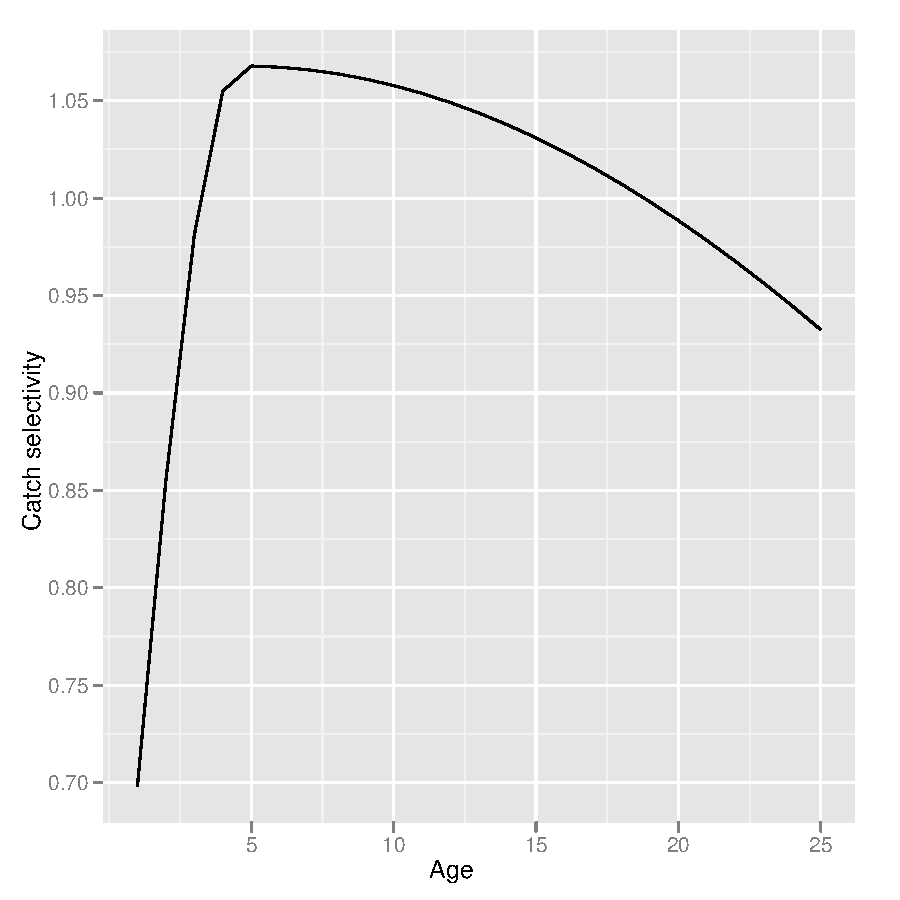
\includegraphics{script-genericSelectivityPlot}
\caption{Double normal catch selectivity curve for the generic stock with parameters $a1=0.5$, $sL=0.5$ and $sR=5$.}
\label{fig:generic_selectivity}
\end{figure}


%*******************************************************************************

\section{Historic stock trajectory}

\subsection{Historic fishing scenarios}

When \cite{Magnusson:2007} where investigating how information content
of the catch and index histories affected the assessment they used four different
scenarios of fishing mortality:

\begin{enumerate}
\item one-way trip, harvest rate gradually increases
\item no change, constant at a somewhat low harvest rate
\item good contrast, stock is fished down to less than half its initial size, then allowed to rebuild
\item rebuild only, stock begins at low abundance and is allowed to rebuild under low fishing mortality
\end{enumerate}


We begin by looking at scenario 3 only: starting from 0, $F$ will increase to $2F^{MSY}$
before decreasing slightly over a period of 40 years (Figure~\ref{fig:Fscenario}). 

\begin{figure}
\centering
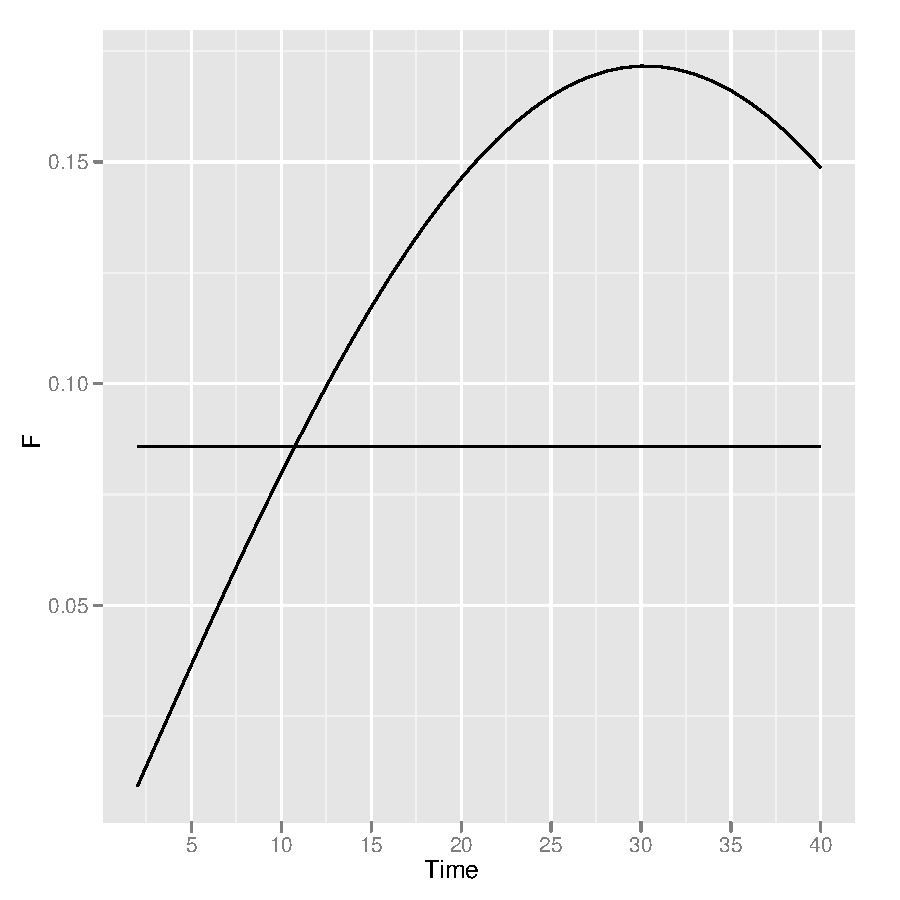
\includegraphics{script-F_plot1}
\caption{Fishing mortality scenario. $F$ increases from 0 to $2F^{MSY}$. The horizontal line is $F^{MSY}$.}
\label{fig:Fscenario}
\end{figure}

\subsection{Historic biomass trajectory}

Using the glory of $FLash$ we can now project the stock forward from time $t=0$ to $t=40$ under this fishing
scenario. To perform our projection we convert our generic stock (currently a $FLBRP$ object) into an $FLStock$ object,
define an $FLQuant$ containing the recruitment residuals, setup a control object and then project forward:


The resulting stock object can be seen in Figure~\ref{fig:hist_proj}.

\begin{figure}
\centering
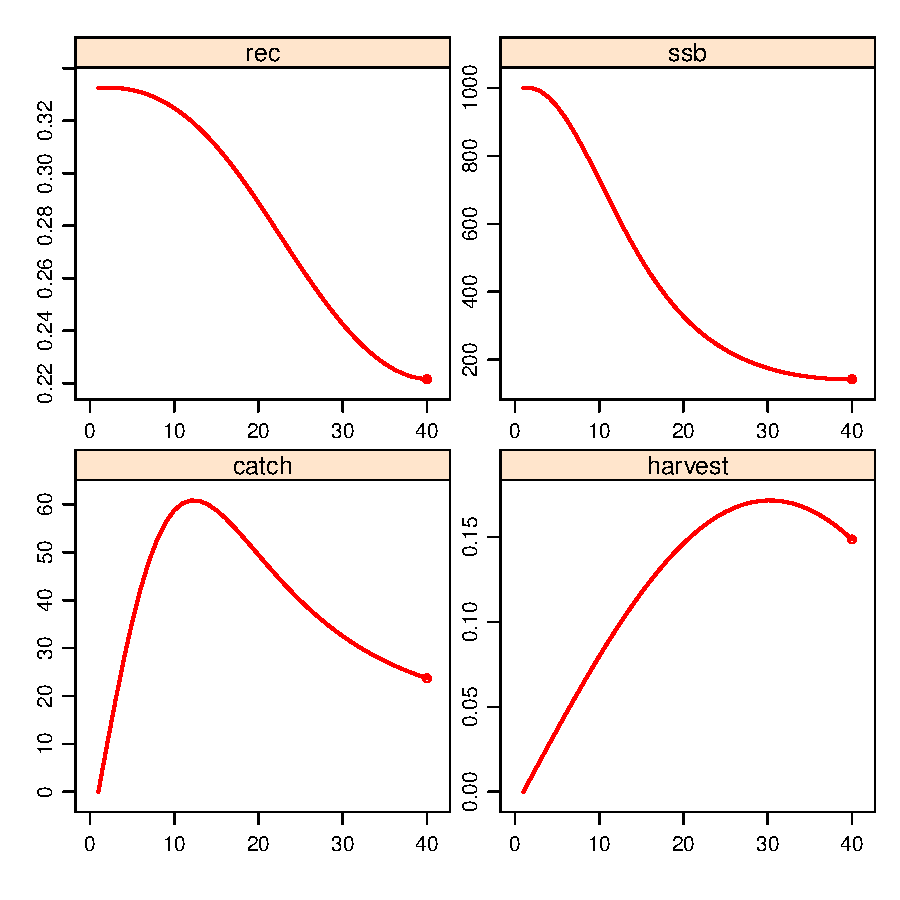
\includegraphics{script-hist_proj_plot}
\caption{Historic stock dynamics}
\label{fig:hist_proj}
\end{figure}

\section{Management strategy projection}

\subsection{Management scenarios}

We compared three different managment scenarios:
\begin{enumerate}
\item perfect knowledge
\item model based control rule
\item empirical control rule
\end{enumerate}

Management objectives were specified as a target catch $C^{TAR} = C^{MSY}$ and biomass $B^{TAR} = B^{MSY}$. 
Note that both targets are consistent with each other (i.e. it is feasible to achive both simultaneously).

The harvest conrol rule defines the catch per year
\[
C_{y+1} = \frac{C^{TAR}G(B_y)}{G(B^{TAR})}
\]
where $G(B)$ is our observation of the resource. For the scenarios listed above:
\begin{enumerate}
\item $G(B) = B$
\item $G(B) = \hat{B}$
\item $G(B) = I$
\end{enumerate}

To ensure comparibility of results, for all scenarios the values of $C^{TAR}$ and $B^{TAR}$ were assumed known. 
For scenario 3, we observe the survey catch rate $I$ only. Since the survey and commercial catches are obtained under differing
selectivity assumptions $G(B^{TAR}) = I^{TAR} \neq qB^{TAR}$. Instead we calculate $I^{TAR}$ directly from the numbers vector $N^{TAR}_a$
associated with $B^{TAR}$ and assuming a constant survey catchability. Thus $I^{TAR} = q\sum_a{w_a N^{TAR}_a}$.

Since scenario 2 requires an estimation step, we predict that as survey effort declines performance of this control rule will deteriorate.
Specifically it will deteriorate at a faster rate than the control rule in scenario 3, which is empirical. Performance was measured as the 
probability of $C\geq C^{TAR}$ and $B\geq B^{TAR}$ after a 40 year projection period. Managment scenarios will be compared by a regression of 
performance against survey effort. 


\subsection{Getting the index data for the control rule}

We assume the index comes from a survey vessel, and that the resource is fully selected by the gear. 
We use empirical survey data to estimate the relationship between uncertainty in our catch rate index and the survey effort. Specifically, data
were extracted from the ICES International Bottom Trawl Survey (IBTS) database for the North Sea, and filtered for \textit{Gadus morhua} and the GOV gear type.
For each year from 1983 to 2011, bootstrap samples of individual trawls were taken, from which a mean catch rate in numbers per tow ($\hat{I}$) could
be estimated. The number of bootstrap samples represented the hypothesised survey effort. For each year and survey effort, we sampled 1000 values of $\hat{I}$
from the data, from which we obtained the coefficient of variation (Figure~\ref{fig:effCV}).


\begin{figure}
\centering
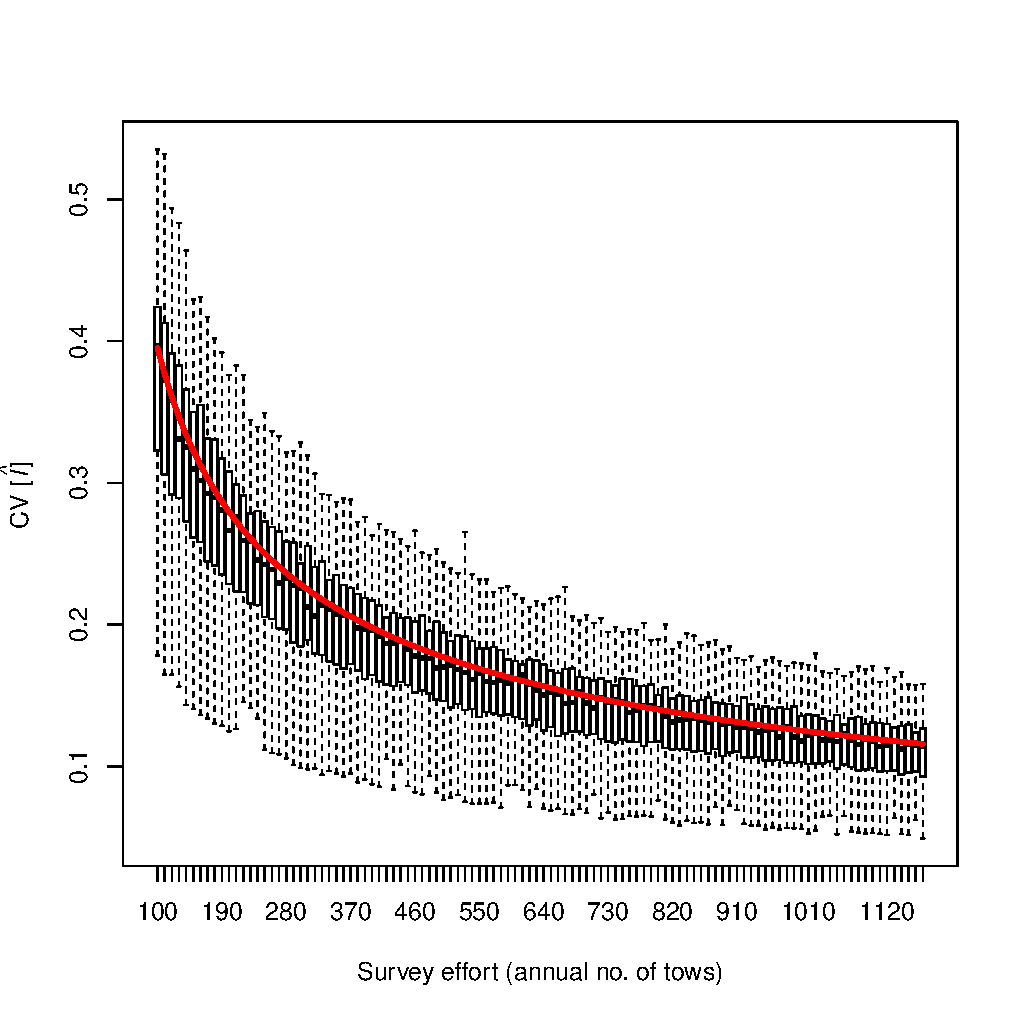
\includegraphics{../dat/effCV.pdf}
\caption{Estimated relationship between CV of the estimated catch rate and survey effort. Boxplots represent the variation across years. 
The mean across years is represented by the fitted red line $\hat{CV}[\hat{I}] = \alpha E ^ \beta$, where $E$ is the survey effort,
$alpha=3.93$ and $\beta = -0.5$.}
\label{fig:effCV}
\end{figure} 


We assume that the survey takes place at the beginning of the year (before any catches have been taken)
and with a constant catchability $q=1e-04$. 

\subsection{Stochasticity}


Sources of stochasticity were as follows:
\begin{enumerate}
\item recruitment: multiplicative log-normal noise around the predicted recruitment
\item observation: the survey catch rate was subjected to a degree of noise equivalent to that given in Figure~\ref{fig:effCV}
for a specified level of effort
\end{enumerate}

\section{Preliminary runs}

We ran deterministic projections for all three management scenarios to ensure that they are behaving as expected (i.e. converging on $B^{TAR}$ and $C^{TAR}$).
These are shown in Figures~\ref{fig:hcr_proj_biomass_sc1}, \ref{fig:hcr_proj_biomass_sc2} and \ref{fig:hcr_proj_biomass_sc3}.

\begin{Schunk}
\begin{Sinput}
> source("../cde/sra.r")
> index <- quantSums(sweep(stock.n(stk2) * stock.wt(stk2), 1, catch.sel(gen1), "*"))
> fit <- optim(SSB0, fn = logl, catch = catch(stk2)[, 1:maxt], index = index[, 1:maxt], hh = slope, 
+     M = m(gen1), mat = mat(gen1), sel = landings.sel(gen1), wght = stock.wt(gen1), amin = range(gen1)["min"], 
+     amax = range(gen1)["max"], method = "L-BFGS-B", lower = c(800), upper = c(1500), hessian = T)
> out <- pdyn(B0 = fit$par, catch = catch(stk2)[, 1:maxt], index = index[, 1:maxt], hh = slope, 
+     M = m(gen1), mat = mat(gen1), sel = landings.sel(gen1), wght = stock.wt(gen1), amin = range(gen1)["min"], 
+     amax = range(gen1)["max"])
> msy <- msy.sra(B0 = fit$par, catch = catch(stk2)[, 1:maxt], index = index[, 1:maxt], hh = slope, 
+     M = m(gen1), mat = mat(gen1), sel = landings.sel(gen1), wght = stock.wt(gen1), amin = range(gen1)["min"], 
+     amax = range(gen1)["max"])
> CTAR <- msy$MSY
> BTAR <- msy$MSY/msy$F
\end{Sinput}
\end{Schunk}

\subsection{Scenario 1: perfect knowledge}


\begin{figure}
\centering
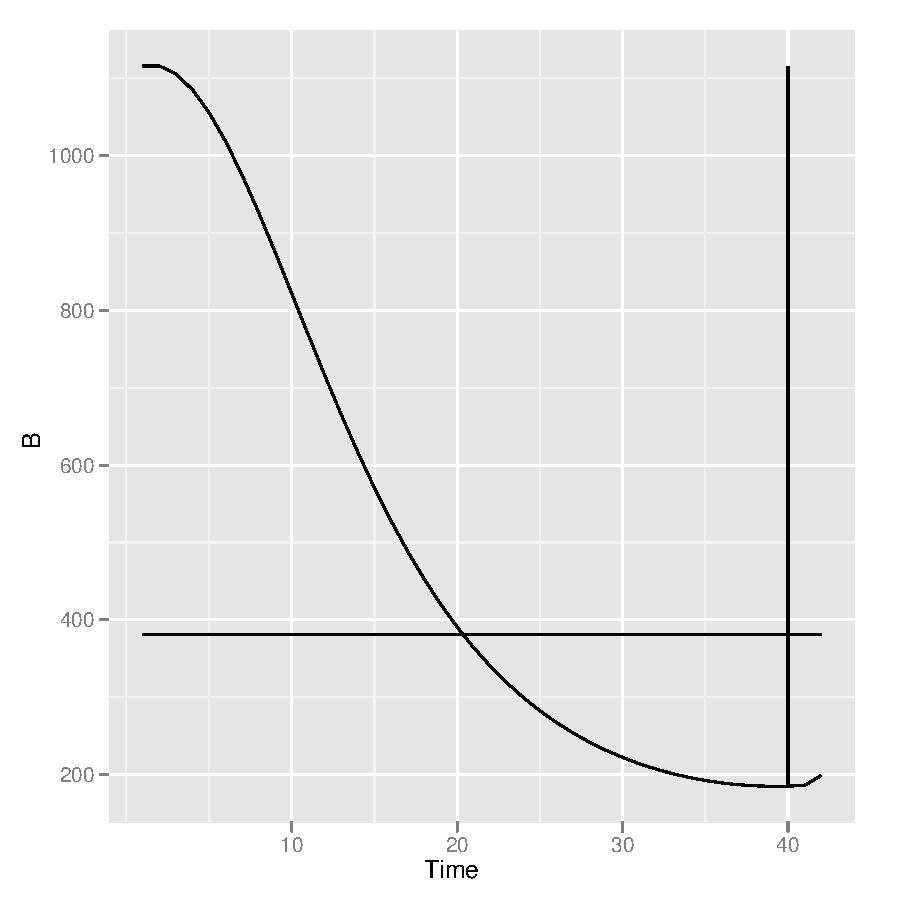
\includegraphics{script-hcr_plot_sc1}
\caption{Scenario 1: Performance of control rule assuming perfect knowledge of resource status. Vertical line represents start of projection period. 
Horizontal line represents the target biomass $B^{TAR}$.}
\label{fig:hcr_proj_biomass_sc1}
\end{figure}

\subsection{Scenario 2: model based control rule}


\begin{figure}
\centering
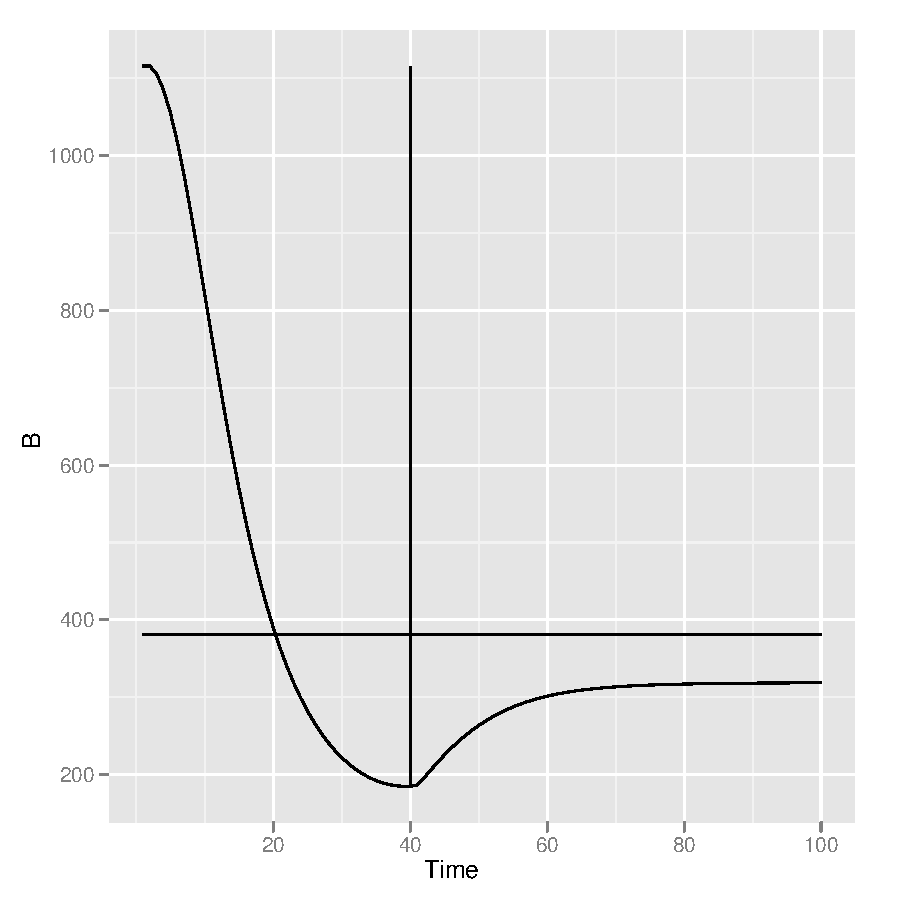
\includegraphics{script-hcr_plot_sc2}
\caption{Scenario 2: Performance of model-based control rule. Vertical line represents start of projection period. 
Horizontal line represents the target biomass $B^{TAR}$.}
\label{fig:hcr_proj_biomass_sc2}
\end{figure}


\subsection{Scenario 3: empirical control rule}


\begin{figure}
\centering
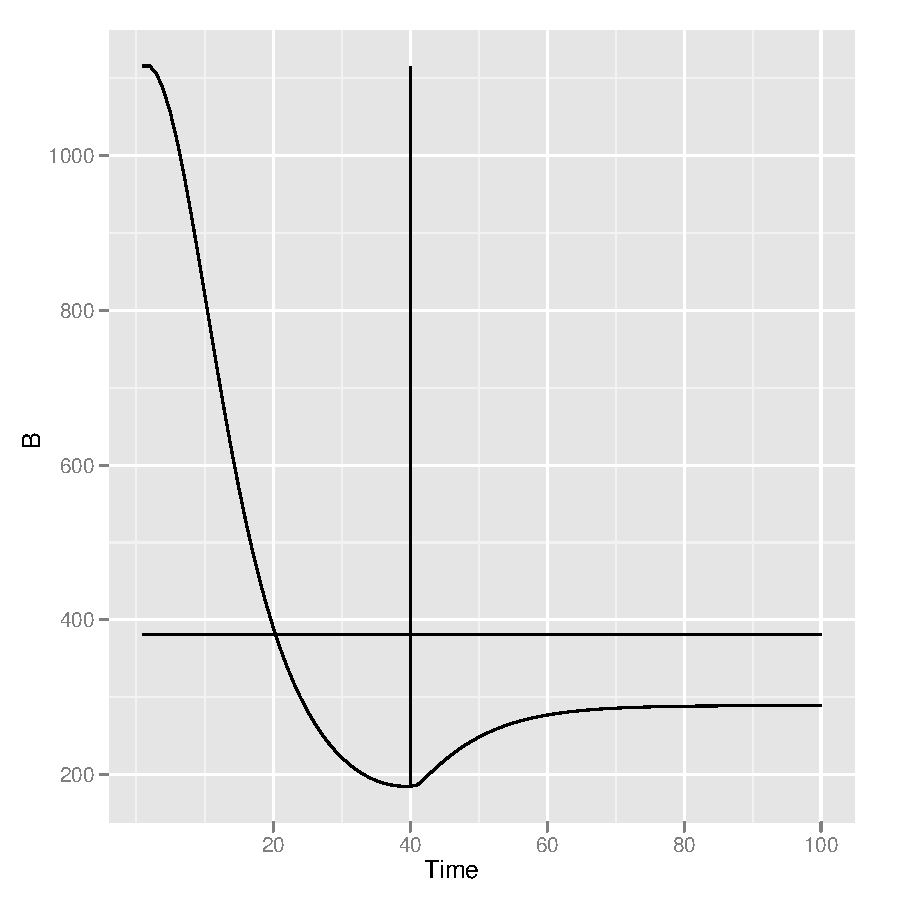
\includegraphics{script-hcr_plot_sc3}
\caption{Scenario 3: Performance of empirical control rule. Vertical line represents start of projection period. 
Horizontal line represents the target biomass $B^{TAR}$.}
\label{fig:hcr_proj_biomass_sc3}
\end{figure}

\section{Stochastic results}

\subsection{Scenario 1}




\newpage
\bibliography{lib}

R
FLR
Sweave
Polacheck


\end{document}

